\chapter{Concurrency Models: Threads, Readiness and Completion}\label{ch:conc}

\begin{objectives}
\begin{itemize}
\item build a cost model for thread-per-connection (stack memory, context switches) and evaluate it with measured numbers;
\item prove that \cc{select}/\cc{poll} cost $\Theta(n)$ per call and that \cc{epoll}/\cc{kqueue} cost $\Theta(1+r)$, and check both against a benchmark;
\item distinguish the reactor and proactor patterns, and say which one \cc{score::net::EventLoop} is;
\item explain io\_uring's submission and completion rings;
\item map v1, v2 and v3 of the roadmap onto the \cc{EventLoop} interface and its limits.
\end{itemize}
{\small\color{muted}\textbf{Chapter references:} Kegel~\cite{kegel1999c10k}; Banga et al.~\cite{banga1999scalable}; Lemon~\cite{lemon2001kqueue};
Schmidt~\cite{schmidt1995reactor}; Pyarali et al.~\cite{pyarali1997proactor}; POSA2~\cite{schmidt2000posa2};
Axboe~\cite{axboe2019iouring}; Kerrisk~\cite{kerrisk2010tlpi}.}
\end{objectives}

\section{The question: how does one process serve \texorpdfstring{$n$}{n} connections?}
A connection spends nearly all its life waiting: for the client to send, for the kernel to free buffer space, for a
disk. Concurrency models differ in \emph{who waits} and \emph{what waiting costs}. There are three families:
\begin{enumerate}[label=\textbf{\color{yel}(\roman*)}]
\item \textbf{One thread per connection.} Each thread blocks in \cc{recv}; the kernel scheduler is the event loop.
\item \textbf{Readiness notification (reactor).} One thread asks the kernel ``which of my descriptors can make progress?'' and performs non-blocking I/O on those.
\item \textbf{Completion notification (proactor).} The thread submits operations; the kernel performs them and reports ``this read finished, here are the bytes''.
\end{enumerate}

\begin{history}
In 1999 Dan Kegel's web page ``The C10K problem''~\cite{kegel1999c10k} asked how to serve ten thousand concurrent clients
from one machine, and catalogued the then-available strategies. At the time the dominant Apache configuration,
the \emph{prefork} model, dedicated a whole process to each connection. Banga, Mogul and Druschel had just shown that
\cc{select}'s per-call cost made event-driven servers scale poorly and proposed an explicit event-delivery
interface~\cite{banga1999scalable}. FreeBSD's \cc{kqueue} (Lemon, 2001)~\cite{lemon2001kqueue} and Linux's \cc{epoll}
(merged during the 2.5 development series, first stable in 2.6) followed. nginx, publicly released by Igor Sysoev in 2004,
was built around such an event loop from the start. \Cref{sec:hist-c10k} returns to this history.
\end{history}

\section{Thread-per-connection: the cost model}\label{sec:tpc}
\begin{layman}
A restaurant can give every table its own waiter. Service is simple, since each waiter only thinks about one table, but
waiters stand idle most of the evening, every one of them needs a uniform and a locker, and when twenty waiters crowd the
kitchen door they spend their time getting out of each other's way.
\end{layman}

Let $n$ be the number of connections. Each thread needs a stack (virtual address space reserved up front, physical
pages committed on first touch) and kernel bookkeeping, and each request wakes a thread, which costs a context switch.

\begin{definition}[Thread-per-connection cost model]\label[definition]{def:tpcmodel}
With reserved stack size $S$, resident stack $s\le S$, per-thread kernel overhead $\kappa$, service time $w$ per request and
context-switch cost $\sigma$, a thread-per-connection server needs virtual memory $V(n)=nS$, resident memory
$M(n)\approx n(s+\kappa)$, and on one core can complete at most
\[ \lambda_{\max}=\frac{1}{w+2\sigma} \]
requests per second, counting one switch to wake the handler and one to leave it.
\end{definition}

\begin{verified}
Measured on the machine described on the title page (\file{verify/layout.cpp}, \file{verify/bench.cpp}):
\begin{itemize}
\item default \cc{pthread} stack for a secondary thread: \textbf{524{,}288 bytes (512 KiB)}; \cc{ulimit -s} for the main thread: \textbf{8176 KiB};
\item \cc{std::thread} create + join: \textbf{14.9\,\textmu s} (mean of 20{,}000);
\item one blocking hand-off between two threads over a pipe (half a ping-pong round trip): \textbf{2.3\,\textmu s} (mean of 200{,}000 round trips of 4.5\,\textmu s).
\end{itemize}
\end{verified}

With $S=512$\,KiB, $10^4$ threads reserve $4.88$\,GiB of address space; with the 8\,MiB default common on Linux, $78.1$\,GiB.
Reservation is not residence, so the machine survives, but the numbers explain why thread-per-connection servers lower
the stack size. The switching term matters more: if $w$ is a few microseconds of VaR arithmetic on cached data, then
$2\sigma\approx 4.6$\,\textmu s is the same order as the useful work.

\section{Readiness APIs and their asymptotics}
\subsection{select and poll: the interest set travels on every call}
\cc{poll(fds, n, timeout)} receives an array of $n$ descriptors each time it is called. \cc{select} does the same with
bitmaps limited to \cc{FD_SETSIZE} descriptors (1024 on this system, verified by compiling a one-line program).

\begin{proposition}[Linear cost of stateless readiness]\label[proposition]{prop:polln}
Any implementation of \cc{poll} that holds no state between calls takes $\Omega(n)$ time per call, even if only one
descriptor is ready.
\end{proposition}
\begin{proof}
The result must report \cc{revents} for every entry, and the input may differ arbitrarily from the previous call. An
implementation that skipped entry $i$ could not distinguish an input where descriptor $i$ is ready from one where it is
not, so it would be wrong on one of them. Hence every entry is read, and copying the array from user memory alone is $\Theta(n)$.
\end{proof}

\subsection{epoll and kqueue: the interest set lives in the kernel}
\cc{epoll_ctl} and \cc{kevent} \emph{register} interest once. The kernel attaches a callback to each watched file, and
when a file becomes ready the callback appends it to a ready list. \cc{epoll_wait} and \cc{kevent} only drain that list.

\begin{theorem}[Cost of stateful readiness]\label{thm:epoll}
If registering and deregistering a descriptor costs $O(1)$ amortized, and each readiness transition costs $O(1)$ to record,
then a wait that returns $r$ ready descriptors costs $\Theta(1+r)$, independent of the number $n$ of registered descriptors.
\end{theorem}
\begin{proof}[Proof sketch]
The wait performs constant work to check the ready list and $O(1)$ per element it copies out, giving $O(1+r)$. It must at least
write $r$ results, giving $\Omega(1+r)$. The $n$ idle descriptors are never touched by the wait: their cost was paid once
at registration and is charged to \cc{epoll_ctl}/\cc{kevent} calls, not to waits. Summed over a run, total work is
$O(\#\text{registrations}+\#\text{transitions}+\sum r)$.
\end{proof}

The prediction is easy to test: register $n$ pipes, make exactly one readable, and time a zero-timeout wait.
\Cref{fig:pollbench} shows the result.

\begin{figure}[htbp]
\centering
\begin{tikzpicture}
\begin{loglogaxis}[darkaxis,width=0.92\linewidth,height=7.2cm,
  xlabel={registered descriptors $n$ (one ready)},ylabel={time per call (\textmu s)},
  grid=major,legend pos=north west,xmin=0.8,xmax=12000,ymin=0.1,ymax=3000]
\addplot[color=red,mark=*,mark size=1.8pt,thick] table[x=n,y=poll_us]{data/bench.dat};
\addlegendentry{\texttt{poll()} (interest set copied each call)}
\addplot[color=grn,mark=square*,mark size=1.8pt,thick] table[x=n,y=kqueue_us]{data/bench.dat};
\addlegendentry{\texttt{kevent()} on a \texttt{kqueue} (registered once)}
\addplot[color=muted,dashed,domain=1:10000,samples=2] {0.1394*x};
\addlegendentry{fit: $0.139\,n$ \textmu s}
\end{loglogaxis}
\end{tikzpicture}
\caption{Measured cost of one readiness check on macOS (Apple M3 Max), median of five runs of 2000 calls
(\file{verify/bench.cpp}). \texttt{poll} grows linearly, about 0.139\,\textmu s per descriptor (least-squares fit);
\texttt{kevent} stays near 0.19--0.24\,\textmu s from $n=1$ to $n=8000$.}
\label{fig:pollbench}
\end{figure}

\begin{center}
\small
\begin{tabular}{@{}rrrr@{}}
\toprule
\textcolor{muted}{$n$} & \textcolor{muted}{\texttt{poll} (\textmu s)} & \textcolor{muted}{\texttt{kevent} (\textmu s)} & \textcolor{muted}{ratio}\\
\midrule
1 & 0.386 & 0.197 & 2.0\\
100 & 11.378 & 0.200 & 57\\
1000 & 134.507 & 0.197 & 683\\
8000 & 1106.619 & 0.200 & 5533\\
\bottomrule
\end{tabular}
\end{center}

\subsection{Level- versus edge-triggered}
In \emph{level-triggered} mode (the default for both APIs) a descriptor is reported on every wait while it remains readable.
In \emph{edge-triggered} mode (\cc{EPOLLET}, \cc{EV_CLEAR}) it is reported once per transition from not-ready to ready.

\begin{pitfall}[title={Pitfall: edge-triggered without draining}]
With edge triggering, a handler that reads 4096 bytes and returns while more bytes sit in the socket buffer will
not be told again until \emph{new} data arrives. If the client is waiting for a reply before sending more, both sides
wait forever. Under edge triggering the rule is: read until \cc{EAGAIN}, and feed everything to the codec.
\Cref{ex:et} asks you to prove the deadlock.
\end{pitfall}

\section{Reactor and proactor}
Schmidt named the readiness pattern the \emph{Reactor}~\cite{schmidt1995reactor}; Pyarali, Harrison, Schmidt and Jordan
named the completion pattern the \emph{Proactor}~\cite{pyarali1997proactor}; both are catalogued in
POSA2~\cite{schmidt2000posa2}.

\begin{definition}[Reactor]\label[definition]{def:reactor}
An event loop that demultiplexes \emph{readiness} events on a set of handles and synchronously dispatches each to a
registered handler, which then performs the I/O itself without blocking.
\end{definition}
\begin{definition}[Proactor]\label[definition]{def:proactor}
An event loop in which handlers \emph{initiate} asynchronous operations, the operating system performs them, and the loop
dispatches \emph{completion} events, carrying results, to completion handlers.
\end{definition}

\begin{figure}[htbp]
\centering
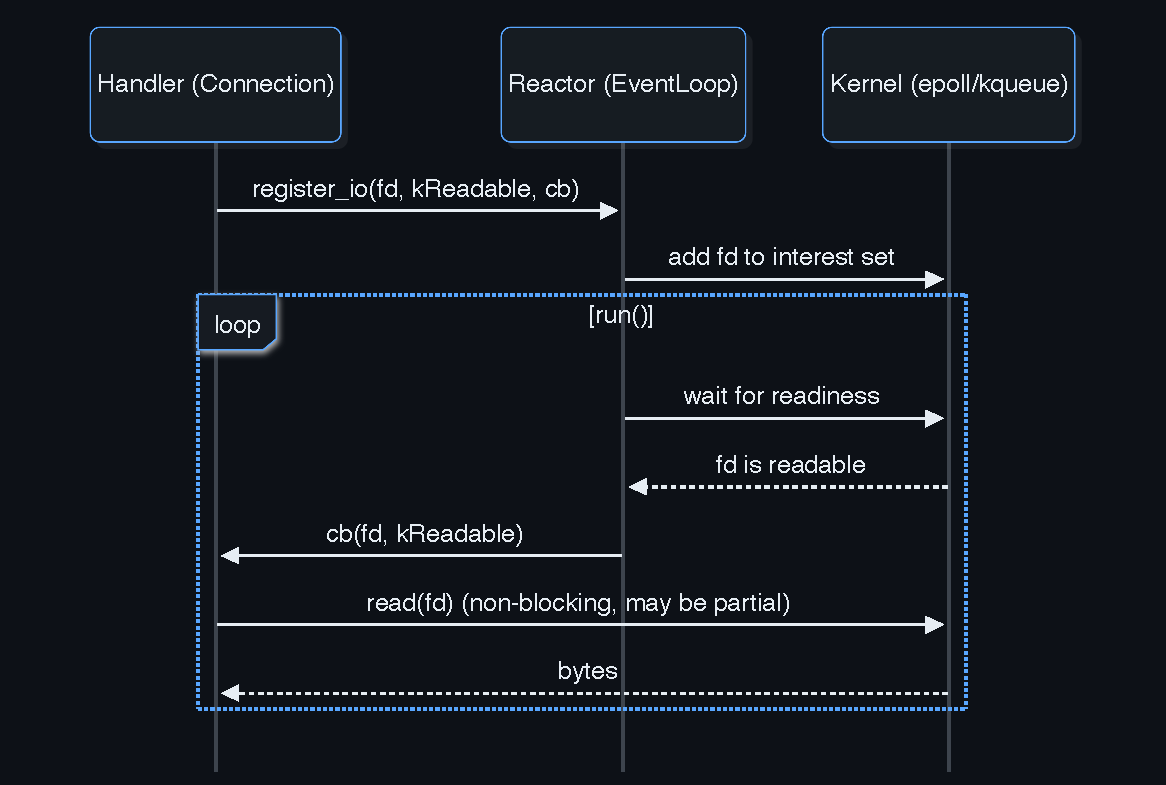
\includegraphics[width=0.66\linewidth]{diagrams/reactor_seq.pdf}\\[-1pt]
{\small\color{muted}(a) Reactor: ``you may read now''.}\\[6pt]
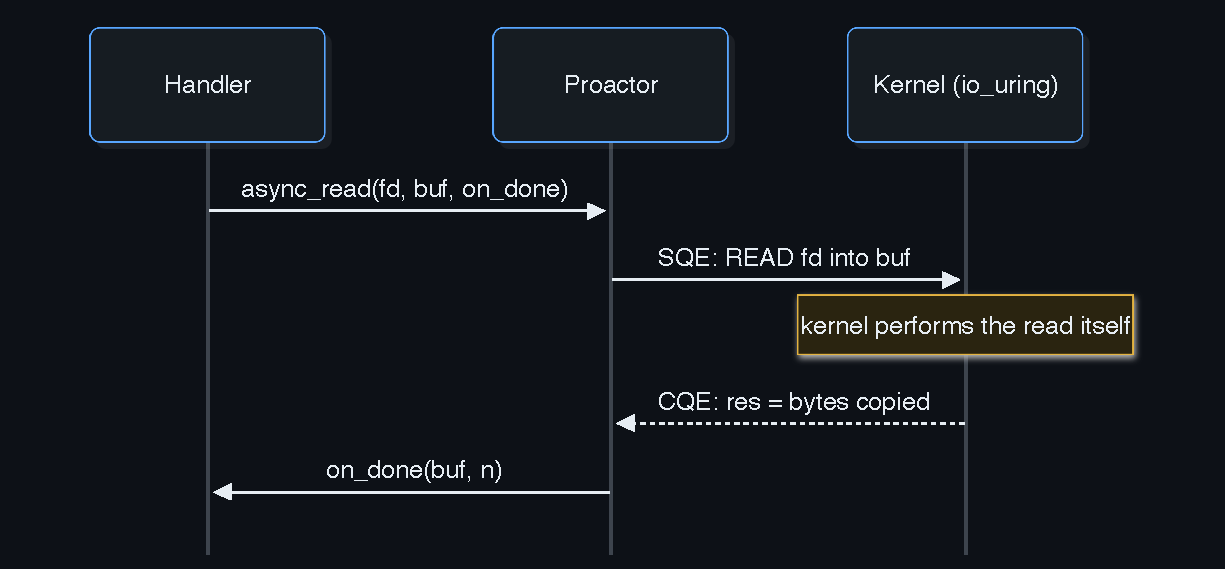
\includegraphics[width=0.6\linewidth]{diagrams/proactor_seq.pdf}\\[-1pt]
{\small\color{muted}(b) Proactor: ``your read is done''.}
\caption{Readiness versus completion (Mermaid). In (a) the handler performs the copy; in (b) the kernel does, into a
buffer the handler supplied when it submitted the operation.}
\label{fig:reactorproactor}
\end{figure}

\repo[firstline=5,lastline=34]{include/score/net/event_loop.hpp}{\cc{EventLoop} is a \emph{reactor} interface:
\cc{register_io(fd, event, cb)} subscribes to readiness, and \cc{IoCallback} receives only \cc{(fd, event)}, no bytes and
no byte count. A completion backend must therefore either emulate readiness or the interface must grow
(\cref{ex:uringadapt}).}{lst:eventloop}

\section{io\_uring: shared rings}
io\_uring, designed by Jens Axboe and merged in Linux 5.1 (2019)~\cite{axboe2019iouring}, replaces one system call per
operation with two ring buffers in memory shared between the process and the kernel. The application writes
\emph{submission queue entries} (SQEs) at the tail of the SQ; the kernel consumes them from the head, performs the
operations, and writes \emph{completion queue entries} (CQEs) to the CQ, which the application consumes.

\begin{figure}[htbp]
\centering
\begin{tikzpicture}[x=0.9cm,y=0.9cm]
  % SQ
  \node[font=\small\bfseries,text=acc] at (3.5,2.0) {Submission queue (SQ)};
  \foreach \i in {0,...,7}{\draw[draw=acc,fill=codebg] (\i,0.6) rectangle ++(1,0.9);}
  \foreach \i/\t in {2/READ,3/READ,4/WRITE}{\fill[acc!35!codebg] (\i+0.04,0.64) rectangle ++(0.92,0.82); \node[font=\scriptsize\ttfamily,text=fg] at (\i+0.5,1.05) {\t};}
  \draw[-{Stealth},thick,yel] (2.0,-0.1) node[below,font=\scriptsize,text=yel]{head (kernel)} -- (2.0,0.55);
  \draw[-{Stealth},thick,grn] (5.0,-0.1) node[below,font=\scriptsize,text=grn]{tail (app)} -- (5.0,0.55);
  % CQ
  \node[font=\small\bfseries,text=org] at (13.0,2.0) {Completion queue (CQ)};
  \foreach \i in {0,...,7}{\draw[draw=org,fill=codebg] (9.5+\i,0.6) rectangle ++(1,0.9);}
  \foreach \i/\t in {1/res=44,2/res=4096}{\fill[org!35!codebg] (9.5+\i+0.04,0.64) rectangle ++(0.92,0.82); \node[font=\tiny\ttfamily,text=fg] at (9.5+\i+0.5,1.05) {\t};}
  \draw[-{Stealth},thick,grn] (10.5,-0.1) node[below,font=\scriptsize,text=grn]{head (app)} -- (10.5,0.55);
  \draw[-{Stealth},thick,yel] (12.5,-0.1) node[below,font=\scriptsize,text=yel]{tail (kernel)} -- (12.5,0.55);
  % kernel
  \node[boxn,draw=muted,minimum width=4.8cm] (k) at (8.25,-1.9) {kernel: consume SQEs, perform I/O, post CQEs};
  \draw[arr] (4.0,0.55) to[out=-90,in=150] (k.west);
  \draw[arr] (k.east) to[out=30,in=-90] (12.0,0.55);
  \node[font=\scriptsize,text=muted,align=center] at (8.25,1.05) {shared\\memory};
\end{tikzpicture}
\caption{io\_uring's two single-producer/single-consumer rings (TikZ). The application produces SQEs and consumes CQEs;
the kernel does the reverse. One \texttt{io\_uring\_enter} call can submit many SQEs; in \texttt{SQPOLL} mode a kernel
thread polls the SQ and submission needs no system call at all.}
\label{fig:uring}
\end{figure}

Because each ring has exactly one producer and one consumer, it needs no lock: the producer writes the entry, then
publishes it by storing the new tail with release semantics; the consumer reads the tail with acquire semantics before
reading entries. The cost per operation falls from ``one system call'' to ``a few cache lines'', and the ring also
carries operations that \cc{epoll} cannot express, such as buffered file reads.

\section{The cost table}
\begin{center}
\footnotesize
\begin{tabularx}{\linewidth}{@{}>{\leavevmode\bfseries\color{yel}}p{2.3cm} >{\raggedright\arraybackslash}X >{\raggedright\arraybackslash}p{1.9cm} >{\raggedright\arraybackslash}p{2.1cm} >{\raggedright\arraybackslash}p{2.1cm} >{\raggedright\arraybackslash}p{1.7cm}@{}}
\toprule
\textcolor{muted}{Model} & \textcolor{muted}{Notification} & \textcolor{muted}{Cost per wait} & \textcolor{muted}{Memory} & \textcolor{muted}{Syscalls per I/O} & \textcolor{muted}{\texttt{score}}\\
\midrule
Thread per conn. & scheduler wakes the blocked thread & $\sigma\approx 2.3$\,\textmu s per switch (measured) & $nS$ virtual; $n(s+\kappa)$ resident & 1 (\cc{recv}) & v1, Phase 5\\
\cc{select}/\cc{poll} & readiness, stateless & $\Theta(n)$; $0.139$\,\textmu s$\cdot n$ (measured) & $O(n)$ per call & 1 wait + 1 per I/O & not planned\\
\cc{epoll}/\cc{kqueue} & readiness, kernel-held interest set & $\Theta(1+r)$; $\approx0.2$\,\textmu s (measured) & $O(n)$ once & 1 wait + 1 per I/O & v2, Phase 6 (Linux)\\
io\_uring & completion, shared rings & $\Theta(1+r)$ & rings + buffers & $\le 1$ per batch; 0 with \texttt{SQPOLL} & v3, Phase 7 (stretch)\\
\bottomrule
\end{tabularx}
\captionof{table}{Concurrency models compared. Measured figures are from this machine and are indicative only.}\label{tab:costs}
\end{center}

\section{Mapping the progression onto \texttt{EventLoop}}
\begin{figure}[H]
\centering
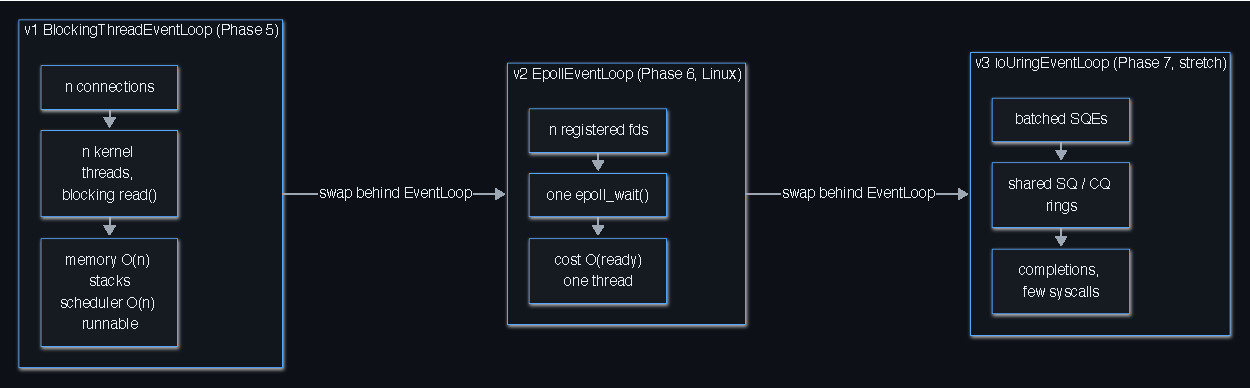
\includegraphics[width=\linewidth]{diagrams/concurrency.pdf}
\caption{The planned v1$\to$v2$\to$v3 progression (Mermaid). Each step replaces one \cc{EventLoop} implementation;
\cc{Server} and \cc{Connection} do not change.}
\label{fig:concprog}
\end{figure}

\begin{figure}[H]
\centering
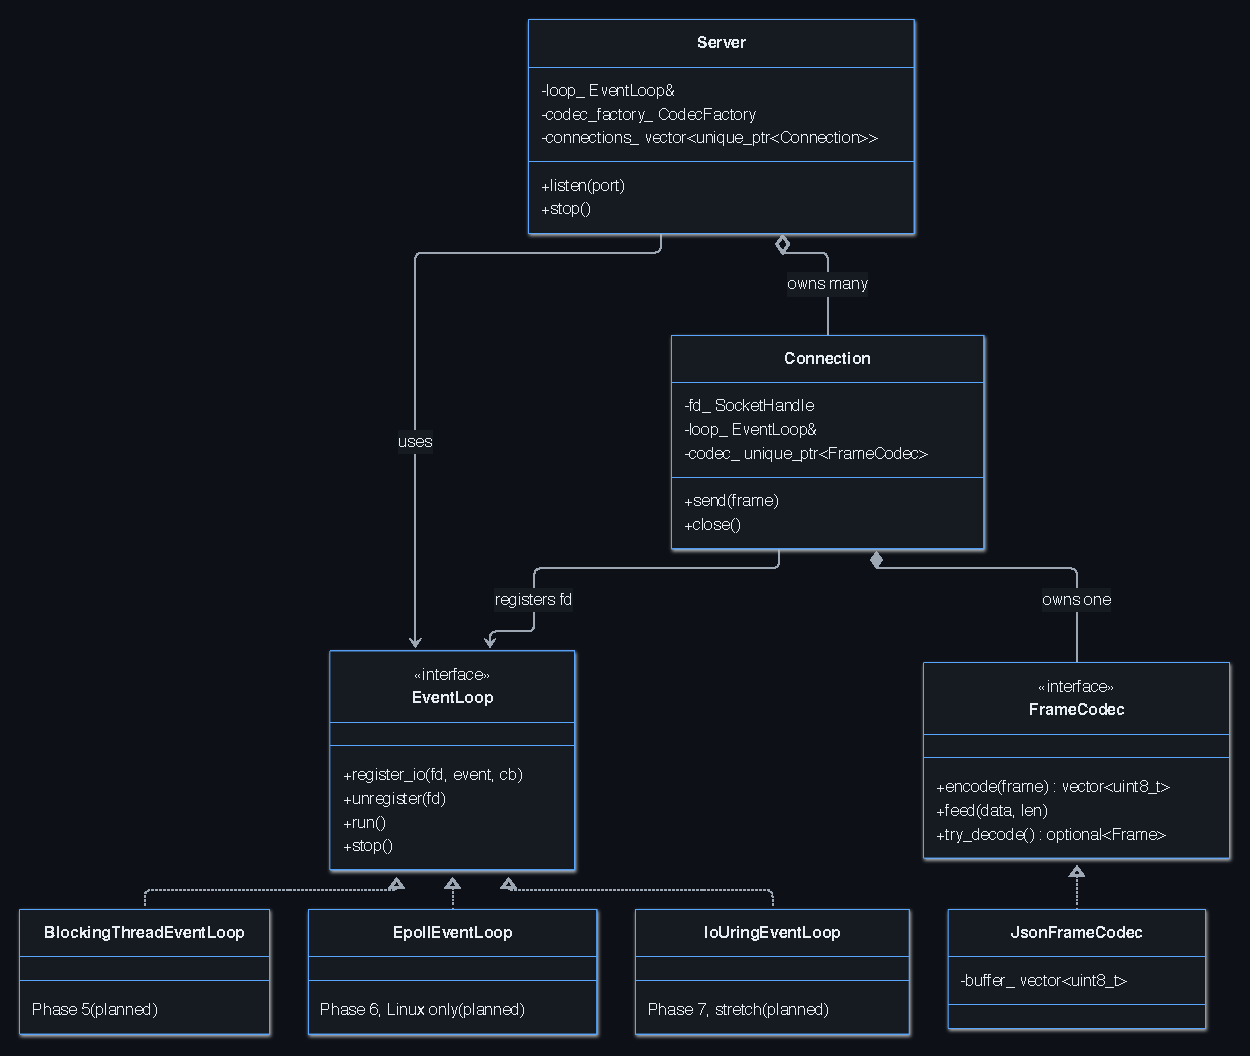
\includegraphics[width=0.8\linewidth]{diagrams/net_classes.pdf}
\caption{\texttt{score::net} class relationships (Mermaid). The three loop implementations are planned (Phases 5--7);
only the interfaces and the \cc{JsonFrameCodec}, \cc{Connection} and \cc{Server} stubs exist today.}
\label{fig:netclasses}
\end{figure}

On macOS there is no \cc{epoll}; the native readiness API is \cc{kqueue}. Decision D4 makes this a matter of adding one
more \cc{EventLoop} implementation rather than a {\ttfamily\color{org}\#ifdef} in \cc{Server}. Phase 4 encodes the same idea in the build:
the \cc{epoll} source is compiled only when CMake reports Linux (\cref{ch:roadmap}).

\begin{exercises}
\ex{ex:pollbudget}{\lvA} Using the fitted slope of \cref{fig:pollbench}, find the $n$ at which a \cc{poll}-based loop
spends half of a 1\,ms tick inside \cc{poll}. Repeat for \cc{kevent} using the measured constant, and explain why the
answer is not a number.

\ex{ex:blocking}{\lvC} \cc{BlockingThreadEventLoop} must implement \cc{register_io(fd, kReadable, cb)}, but a blocking
model has no readiness notification. One design spawns a thread per descriptor that blocks in \cc{recv} and then calls
\cc{cb}. Show that this either loses the bytes it read or requires an interface change, because \cc{IoCallback} carries no
data. Propose the smallest interface change that keeps \cc{Server} unchanged.

\ex{ex:et}{\lvB} Under edge-triggered \cc{epoll}, a handler reads at most 4096 bytes per event and the client has sent
two frames totalling 6000 bytes and then waits for both replies. Prove that the second frame is never decoded. Then
prove that ``read until \cc{EAGAIN}'' removes the deadlock.

\ex{ex:reentrant}{\lvB} A callback invoked by \cc{run()} calls \cc{unregister(fd)} on its own descriptor, or on another
descriptor that is ready in the same batch. Specify semantics for \cc{unregister} that are safe in both cases, and
describe an implementation that never invokes a callback for a descriptor after \cc{unregister} has returned.

\ex{ex:uringadapt}{\lvC} io\_uring can emulate readiness with \cc{IORING_OP_POLL_ADD}. Sketch an
\cc{IoUringEventLoop} that implements the present \cc{EventLoop} interface this way. What does it lose compared with a
true proactor that submits \cc{IORING_OP_RECV}? Would you change the interface instead, and what would that cost the
other two backends?

\ex{ex:memory}{\lvA} Estimate resident memory for $10^4$ idle connections under v1 and v2, assuming 16\,KiB of touched
stack per thread, a 64\,KiB receive buffer in each codec, and 1\,KiB of kernel state per socket. Which term dominates
each model?
\end{exercises}

